\documentclass[twocolumn,a4j]{jsarticle}
\setlength{\topmargin}{-20.4cm}
\setlength{\oddsidemargin}{-10.4mm}
\setlength{\evensidemargin}{-10.4mm}
\setlength{\textwidth}{18cm}
\setlength{\textheight}{26cm}

\usepackage[top=15truemm,bottom=20truemm,left=20truemm,right=20truemm]{geometry}
\usepackage[latin1]{inputenc}
\usepackage{amsmath}
\usepackage{amsfonts}
\usepackage{amssymb}
\usepackage[dvipdfmx]{graphicx}
\usepackage[hang,small,bf]{caption}
\usepackage[subrefformat=parens]{subcaption}
\usepackage[dvipdfmx]{color}
\usepackage{listings}
\usepackage{listings,jvlisting}
\usepackage{geometry}
\usepackage{framed}
\usepackage{color}
\usepackage[dvipdfmx]{hyperref}
\usepackage{ascmac}
\usepackage{enumerate}
\usepackage{tabularx}
\usepackage{cancel}
\usepackage{scalefnt}
\usepackage{overcite}
\usepackage{otf}
\usepackage{multicol}
\usepackage[geometry]{ifsym}
\usepackage{array}

\renewcommand{\figurename}{Fig.}
\renewcommand{\tablename}{Table }

\lstset{
basicstyle={\ttfamily},
identifierstyle={\small},
commentstyle={\smallitshape},
keywordstyle={\small\bfseries},
ndkeywordstyle={\small},
stringstyle={\small\ttfamily},
frame={tb},
breaklines=true,
columns=[l]{fullflexible},
xrightmargin=0zw,
xleftmargin=3zw,
numberstyle={\scriptsize},
stepnumber=1,
numbersep=1zw,
lineskip=-0.5ex
}

% キャプション後ろのダブルコロンを消す
\makeatletter
\long\def\@makecaption#1#2{%
  \vskip\abovecaptionskip
  \iftdir\sbox\@tempboxa{#1\hskip1zw#2}%
    \else\sbox\@tempboxa{#1 #2}%
  \fi
  \ifdim \wd\@tempboxa >\hsize
    \iftdir #1\hskip1zw#2\relax\par
      \else #1 #2\relax\par\fi
  \else
    \global \@minipagefalse
    \hbox to\hsize{\hfil\box\@tempboxa\hfil}%
  \fi
  \vskip\belowcaptionskip}
\makeatother

% タイトル
\makeatletter
\def\@maketitle
{
\begin{center}
{\LARGE \@title \par}
\end{center}
\begin{flushright}
{\large \@date 報告書 No.32}\\
{\large M2 \@author}
\end{flushright}
\par\vskip 1.5em
}
\makeatother

\author{来代 勝胤}
\title{令和4年度 7月 第2週 報告書}
\date{2022/7/13}

\begin{document}
\columnseprule=0.1mm
\maketitle

\section*{報告内容}
\begin{enumerate}[1.]
  \item 三角翼後流の撮影
  \item 車両モデル車軸部の撮影
  \item 可視化情報シンポジウムの資料作成 (1)
  \item 来週の予定
\end{enumerate}

\section*{進捗報告}
今週は可視化情報シンポジウムの資料作成に向けた
二次流れの撮影実験を行った.
三角翼モデルについて渦構造の乱れが少ないと考えられる
後端直後の流れについて,右翼部および中央部の測定と結果の解析を行った.

\section{三角翼後流の撮影}
\begin{table}[hbtp]
  \centering
  \caption{The Experimental Conditions}
  \begin{tabular}{ c r l }
    \hline
    Mainstream velocity              & 250  & mm/s \\ \hline
    Frame rate                       & 800  & fps  \\ \hline
    Shutter speed                    & 1000 & 1/s  \\ \hline
    Thickness of LLS 1               & 1.0  & mm   \\ \hline
    Thickness of LLS 2               & 3.0  & mm   \\ \hline
    Distance between LLS 1 and LLS 2 & 2.5  & mm   \\ \hline
    Shooting time                    & 5    & s    \\ \hline
  \end{tabular}
\end{table}

\subsection{右翼部の撮影結果}
可視化情報シンポジウムの資料作成に向けて
右翼の撮影を再度行った.
これまで,後端部から50 mmの位置について
計測を行ってきたが,外乱による渦構造の変化や崩壊の可能性を考慮し
後端部直後の撮影を行った.
また,撮影時のゲインを変更して計測を行い
その結果をFig.1に示す.\\

\begin{figure}[htbp]
  \footnotesize
  \begin{center}
    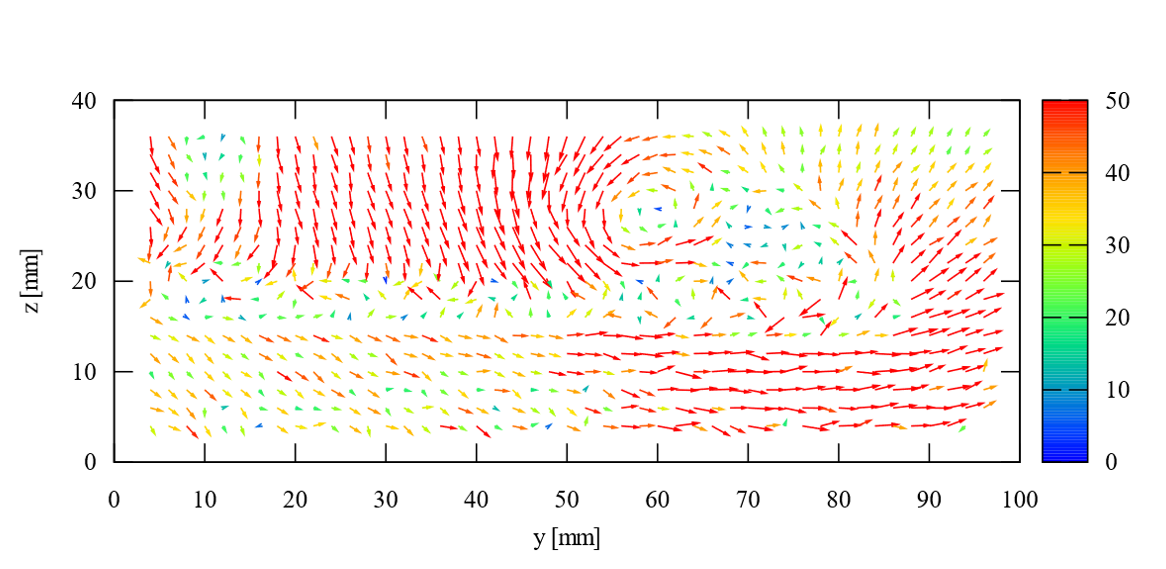
\includegraphics[width=85mm]{../images/right_+0.png}
    \subcaption{Gain $+0$}
    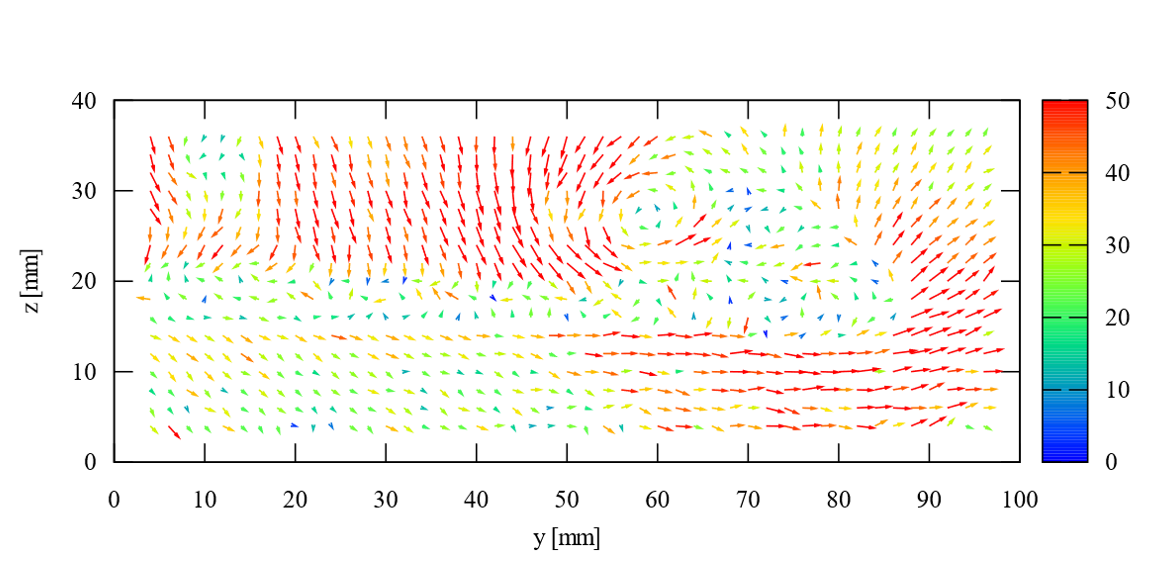
\includegraphics[width=85mm]{../images/right_+5.png}
    \subcaption{Gain $+5$}
    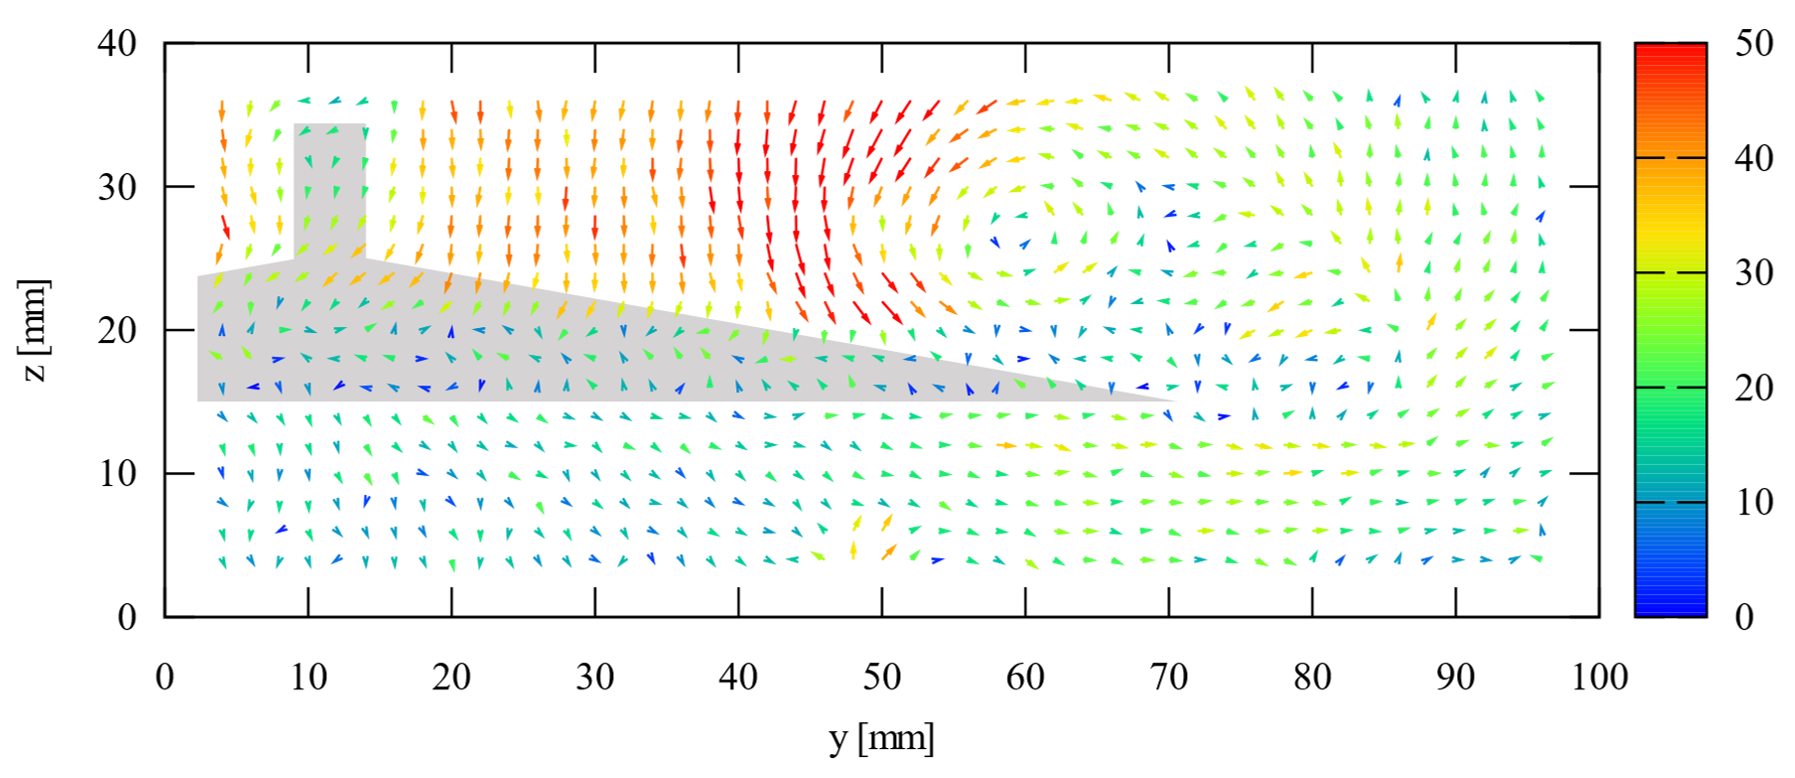
\includegraphics[width=85mm]{../images/right_+10.png}
    \subcaption{Gain $+10$}
  \end{center}
  \caption{PTV time-averaged vectors : $\Delta n = 11$}
\end{figure}

\begin{figure}[htbp]
  \footnotesize
  \begin{center}
    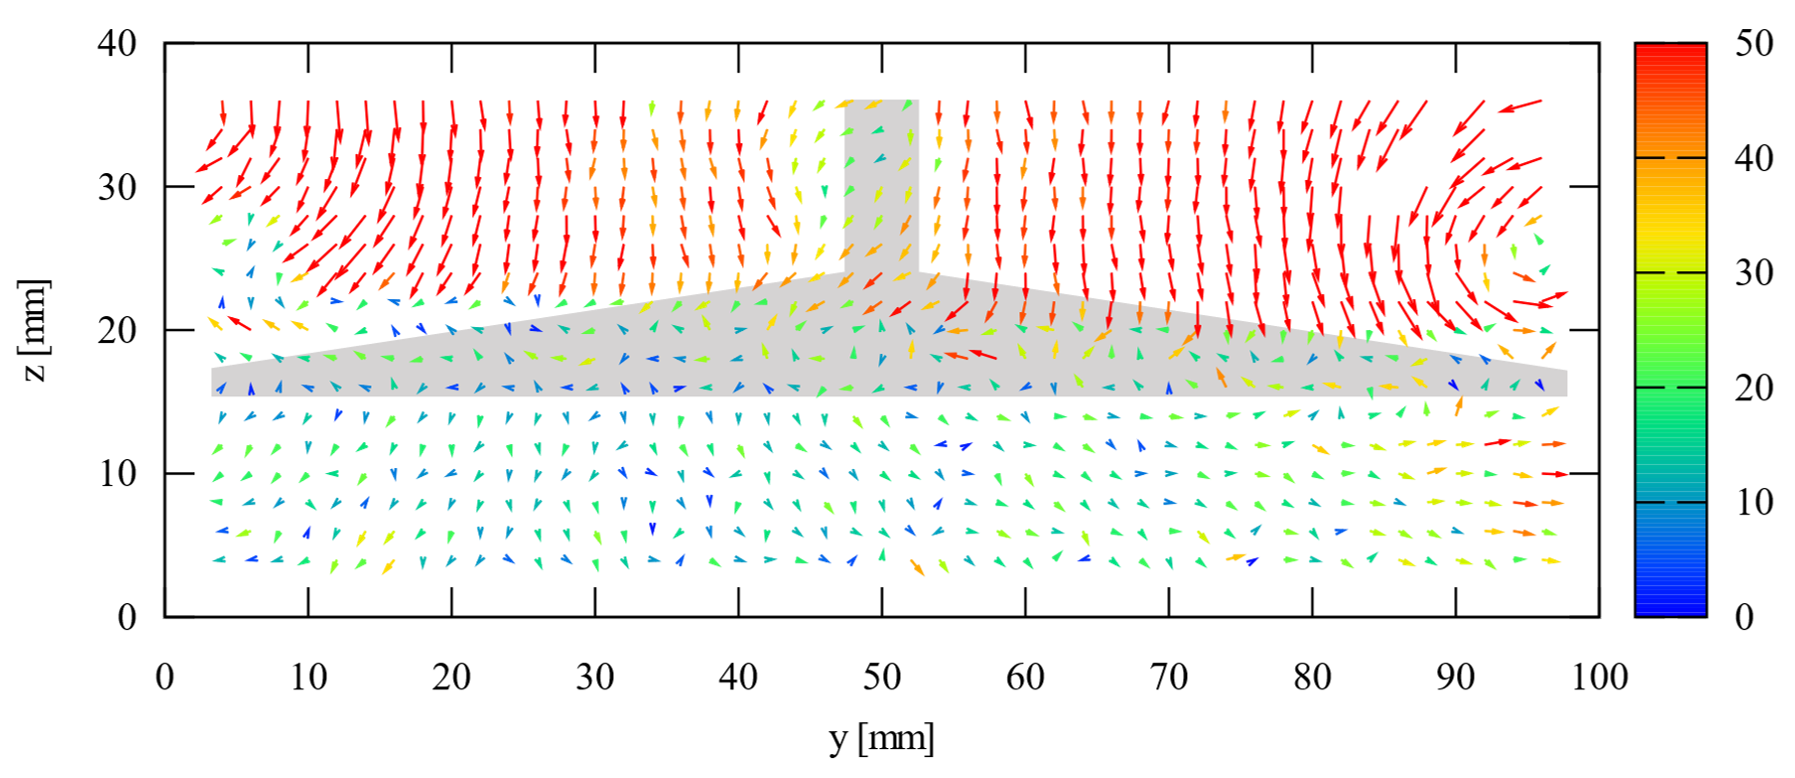
\includegraphics[width=85mm]{../images/center_+5.png}
  \end{center}
  \caption{PTV time-averaged vectors : $\Delta n = 10$, Gain +5}
\end{figure}

\subsection{中央部}
流れの対称性を確認するため,中央部の撮影を行う.
撮影条件は右翼部と同様であり.翼後端直後の撮影を行った.
解析結果をFig.2 に示す.
結果より,中央を境目に対象の流れが発生していることがわかる.

\section{車両モデル車軸部の撮影}
\section{可視化情報シンポジウムの資料作成(1)}

\section{来週の予定}
\begin{itemize}
  \item 実験結果の解析
  \item 粒子追跡プログラムの作成
  \item 可視化情報シンポジウムの資料作成 (2)
\end{itemize}

\end{document}